%% LaTeX Beamer presentation template (requires beamer package)
%% see http://bitbucket.org/rivanvx/beamer/wiki/Home
%% idea contributed by H. Turgut Uyar
%% template based on a template by Till Tantau
%% this template is still evolving - it might differ in future releases!

\documentclass{beamer}

\mode<presentation>
{
\usetheme{Warsaw}

\setbeamercovered{transparent}
}

\usepackage{../../Common/sty/TI84} %TODO: How to get the link working...?



\title{Masterclass programmeren op de GR TI-84 (les 1)}

%\subtitle{}

% - Use the \inst{?} command only if the authors have different
%   affiliation.
%\author{F.~Author\inst{1} \and S.~Another\inst{2}}
\author{Kevin van As}

% - Use the \inst command only if there are several affiliations.
% - Keep it simple, no one is interested in your street address.
% \institute[Universities of]
% {
% \inst{1}%
% Department of Computer Science\\
% Univ of S
% \and
% \inst{2}%
% Department of Theoretical Philosophy\\
% Univ of E}

\date{\today}


% This is only inserted into the PDF information catalog. Can be left
% out.
\subject{Masterclass GR TI-84 programmeren (les 1)}



% If you have a file called "university-logo-filename.xxx", where xxx
% is a graphic format that can be processed by latex or pdflatex,
% resp., then you can add a logo as follows:

% \pgfdeclareimage[height=0.5cm]{university-logo}{university-logo-filename}
% \logo{\pgfuseimage{university-logo}}



% Delete this, if you do not want the table of contents to pop up at
% the beginning of each subsection:
\AtBeginSubsection[]
{
\begin{frame}<beamer>
\frametitle{Outline}
\tableofcontents[currentsection,currentsubsection]
\end{frame}
}

% If you wish to uncover everything in a step-wise fashion, uncomment
% the following command:

%\beamerdefaultoverlayspecification{<+->}

\begin{document}

\begin{frame}
\titlepage
\end{frame}

% \section{Introductie}

% \subsection[Introduction]{Introduction Masterclass GR-Advanced}

\begin{frame} %TODO: Variable over time
\frametitle{Let me introduce myself\ldots}

\begin{itemize}
  \item Kevin van As (23yr)
  \pause
  \item PhD aan de TUDelft in de Natuurkunde
  \pause
  \item Hobbies:
  \begin{itemize}
  	\item Les geven
  	\item Masterclasses organiseren
  	\pause
  	\item Computer programmeren
  	\pause
  	\item Computer games
  \end{itemize}
\end{itemize}
\end{frame}

\begin{frame}
\frametitle{Wat is de cursus?}
\framesubtitle{Leerdoelen}

Je zult leren:
\begin{itemize}
  \item Je Grafische Rekenmachine (GR) TI-84 beter leren kennen.
  \pause
  \item Leren om programma's (\tiPRGM) voor de GR te schrijven:
  \pause
  \begin{itemize}
    \item ABC-formule
    \pause
    \item Priemgetallen
    \pause
    \item Exactor
    \pause
    \item Grafische tools
    \pause
    \item Games
  \end{itemize}
  \pause
  \item En dit leert je ook inzichten om op de computer te leren programmeren!
\end{itemize}
	
\begin{picture}(1,1)
  	\put(240,43){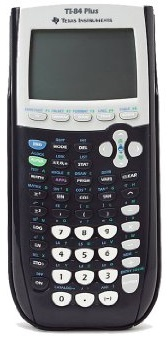
\includegraphics[height=0.3\textheight]{../../Common/figures/TI84.jpg}}
\end{picture}
\end{frame}

\begin{frame}
\frametitle{Wat is de cursus?}
\framesubtitle{Opzet}

\begin{itemize} %TODO: Variable over time
  \item !?!?? Wekelijks op Maandagavond 19:00-21:00.
  \pause
  \item Van DD/MM/YY tot DD/MM/YY, in totaal 5 keer.
  \pause
  \item Les bestaat uit beetje uitleg, en veel zelf proberen.
  \pause
  \item Je krijgt opdrachten mee naar huis om zelf te oefenen.
\end{itemize}

\end{frame}

\begin{frame}
\frametitle{Notatie op deze slides}

Op deze slides zullen we drie verschillende lettertypen vinden.
Het huidige lettertype is normale tekst.

\pause
\tifonttxt{Dit lettertype wordt gebruikt om tekst van je rekenmachine te laten zien.} \inlineticalc{7 \> A: A \! 6}

\pause
Tekens als \tiPRGM, \tiGRAPH, \tiCOS,  \tiXTn\, en \tiENTER\, zijn fysieke knoppen van je rekenmachine.

\pause
En tekens als \tiLOne, \tiACOS, en \tiMATRIX\, zijn knoppen die je met \tiSecond\, kunt bereiken.
Deze knoppen staan boven andere knoppen. Bijvoorbeeld \tiTEST\, is gelijk aan \tiSecond\tiMATH.

\vspace{10 mm}
\visible<5->{
Nu\ldots Laten we beginnen! Rekenmachines bij de hand\ldots
}
\end{frame}


%% END %%

\begin{frame}
\frametitle{Outline}
\tableofcontents
% You might wish to add the option [pausesections]
\end{frame}

% The core pages
\section{Hoe open je een programma?}

\begin{frame}
\frametitle{\tifontbigtxt{NEW} \tiPRGM}

\visible<1-2>{\ticalcfig{\ticalcfigCircle{\ticalcfigCircleColThree}{0.615}}}
\visible<3>{\ticalcfig{\ticalcfigCircleEnter\ticalcfigCircleRight}}
\visible<4>{\ticalcfig{\ticalcfigCircleEnter \ticalcfigCircleAlpha\ticalcfigCircleSecond}}
\visible<5>{\ticalcfig{\ticalcfigCircleSecond\ticalcfigCircle{\ticalcfigCircleColTwo}{0.81}}}

We gaan ons eerste programma aanmaken.
\begin{itemize}
  \item Druk op \tiPRGM.
  \pause %1
  \item \lenitem{Tenzij je eerder een programma hebt gemaakt, zie je alleen \inlineticalc{EXEC \, EDIT \, NEW}.}
  \pause %2
  \item Blader met \tiRight\,naar \tifonttxt{NEW} en druk op \tiENTER.
  \pause %3
  \item \lenitem{Type een naam in. Een prgm naam is maximaal 8 karakters. Druk vervolgens op \tiENTER.}
	  \begin{ticalc}[3.25cm]
	  	PROGRAM\\
	  	NAME=MYPRGM01
	  \end{ticalc}
  
  Merk op dat je een \tiCursorAlpha-cursor hebt: \tiALOCK\,is geactiveerd.
  \pause %4
  \item Sluit het programma nu met \tiQUIT.
\end{itemize}
\end{frame}

\begin{frame}
\frametitle{\tifontbigtxt{EDIT} \tiPRGM}

\visible<1-2>{\ticalcfig{\ticalcfigCircle{\ticalcfigCircleColThree}{0.615}}}
\visible<3>{\ticalcfig{\ticalcfigCircleRight}}
\visible<4>{\ticalcfig{\ticalcfigCircleDown\ticalcfigCircleEnter}}
\visible<5>{\ticalcfig{}}
\visible<6>{\ticalcfig{\ticalcfigCircleAlpha}}

Om het programma nu weer te openen, doe:
\begin{itemize}
  \item Druk op \tiPRGM.
  \pause %1
  \item \lenitem{Je ziet nu een lijst met alle programmas die je kunt uitvoeren.}
	  \begin{ticalc}[3.25cm]
	  	EXEC \, EDIT \, NEW
	  	1:MYPRGM01
	  \end{ticalc}
  \pause %2
  \item Blader met \tiRight\,naar \tifonttxt{EDIT}.
  \pause %3
  \item Hier zie je dezelfde lijst. Gebruik \tiDown\, om naar je programma te bladeren en druk op \tiENTER.
  \pause %4
  \item Als alternatief, kun je ook het nummer intoetsen wat voor je programma staat. Dit is een hotkey om je programma te openen.
  \pause %5
  		Ook kun je met \tiALPHA\, de eerste letter van je programmanaam intoetsen om snel je programma te vinden
  		(indien je later een grotere lijst met programmas hebt dan 1).
\end{itemize}
\end{frame}

\begin{frame}
\frametitle{Deleten/Archiveren van een \tiPRGM}
	TODO?
\end{frame}



%% END %%
\section{Introduction}

\subsection[Introduction]{Introduction Masterclass GR-Advanced}

\begin{frame}
\frametitle{}
\framesubtitle{Subtitles are optional}

\begin{itemize}
  \item
  \item
\end{itemize}
\end{frame}

\begin{frame}
\frametitle{}

% You can create overlays
\begin{itemize}
  \item using the \texttt{pause} command:
  \begin{itemize}
    \item First item.
    \pause
    \item Second item.
  \end{itemize}
  \item using overlay specifications:
  \begin{itemize}
    \item<3-> First item.
    \item<4-> Second item.
  \end{itemize}
  \item using the general \texttt{uncover} command:
  \begin{itemize}
    \uncover<5->{\item First item.}
    \uncover<6->{\item Second item.}
  \end{itemize}
\end{itemize}
\end{frame}


%% END %%
\section{Basic IO}

\subsection{Disp}

\begin{frame}
\frametitle{Het \tifonttxt{PRGM-I/O} menu: input \& output.}

\visible<2>{\ticalcfig{\ticalcfigCircle{\ticalcfigCircleColThree}{0.615}}} % prgm
\visible<3>{\ticalcfig{\ticalcfigCircleRight\ticalcfigCircle{\ticalcfigCircleColThree}{0.615}}} % prgm + right
\visible<4->{\ticalcfig{\ticalcfigCircle{\ticalcfigCircleColThree}{0.615}}} % prgm

We gaan nu een programma tekst laten weergeven.
\begin{itemize}
  \item<2-> \lenitem{Maak zelf een nieuw programma aan: \tifonttxt{DISP1}.}
  \item<3-> \lenitem{Open het programma (\tiPRGM\tiRight\tifonttxt{DISP1}).}
  \item<4-> \lenitem{Druk op \tiPRGM\,om het programmeermenu te openen.}
  \item<5-> \lenitem{Bij menu \tifonttxt{I/O} staat alle Input en Output.}
  \item<6-> We zijn nu geinteresseerd in \tifonttxt{Disp}: ``Display''.
\end{itemize}

\only<4>{
	\begin{ticalc}
		\select{CTL}\,I/O\,EXEC \\
		\selectitem{1\+\:}If \\
		2\:Then \\
		3\:Else \\
		4\:For( \\
		5\:While \\
		6\:Repeat( \\
		7\arrowdown End
	\end{ticalc}
}
\visible<5->{
	\begin{ticalc}
		CTL\,\select{I/O}\,EXEC \\
		1\+\:Input \\
		2\:Prompt \\
		\selectitem{3\:}Disp \\
		4\:DispGraph \\
		5\:DispTable \\
		6\:Output( \\
		7\arrowdown getKey
	\end{ticalc}
}

\end{frame}

\begin{frame}
\frametitle{Hello World!!}

\visible<1-2>{\ticalcfig{\ticalcfigCircle{\ticalcfigCircleColThree}{0.615}}} % prgm
\visible<3>{\ticalcfig{\ticalcfigCircleAlpha\ticalcfigCircleSecond}} % Alpha + 2nd
\visible<4->{\ticalcfig{\ticalcfigCircleAlpha\ticalcfigCircle{\ticalcfigCircleColFive}{0.227}}} % Quote / Mem

We maken nu een ``Hello World'' programma:
\begin{itemize}
  \item<2-> \lenitem{Kies de \tifonttxt{Disp} functie uit het \tifonttxt{I/O} menu.}
  \item<3-> \lenitem{Zet je rekenmachine op \tiALOCK, zodat je letters kunt typen,
  			zonder herhaaldelijk op \tiALPHA\, te drukken.}
  \item<4-> \lenitem{Typ vervolgens \tifonttxt{\qt HELLO\,WORLD\qt} achter \tifonttxt{Disp}.}
  \item<5-> \lenitem{Done! Execute het programma om te testen!}
\end{itemize}

\visible<2->{
	\begin{ticalc}
		CTL\,\select{I/O}\,EXEC \\
		1\+\:Input \\
		2\:Prompt \\
		\selectitem{3\:}Disp \\
		4\:DispGraph \\
		5\:DispTable \\
		6\:Output( \\
		7\arrowdown getKey
	\end{ticalc}
}
\visible<1->{
	\begin{ticalc}[5cm]
		PROGRAM\:DISP1 \\%
		\:\visible<2->{Disp\,\only<4->{\qt HELLO\,WORLD\qt}\only<3->{\tiCursorAlpha}}%
	\end{ticalc}
}

\end{frame}


\subsection{Prompt}

\begin{frame}
\frametitle{Input: \tifontbigtxt{Prompt}}

\begin{itemize}
  \item<1-> Nice\ldots Maar het is veel leuker als de rekenmachine iets meer kan dan alleen ``Hello World'' zeggen.
  \item<2-> \tifonttxt{Prompt} vertelt de rekenmachine iets: Input.
  \item<3-> Bijvoorbeeld, \inlineticalc{Prompt\,A} vraagt de gebruiker om de waarde van de variabele \tifonttxt{A}: een getal.
  \item<4-> Bijvoorbeeld, \inlineticalc{Prompt\,Str1} vraagt de gebruiker om de waarde van de variabele \tifonttxt{Str1}: een string.
\end{itemize}

\visible<2->{
	\begin{ticalc}
		CTL\,\select{I/O}\,EXEC \\
		1\+\:Input \\
		\selectitem{2\:}Prompt \\
		3\:Disp \\
		4\:DispGraph \\
		5\:DispTable \\
		6\:Output( \\
		7\arrowdown getKey
	\end{ticalc}
}

\end{frame}

\begin{frame}
\frametitle{Input: \tifontbigtxt{Prompt}}
\framesubtitle{Meerdere argumenten}

\begin{itemize}
  \item<1-> Merk op dat je meerdere argumenten aan \tifonttxt{Prompt} kunt geven.
  \item<2-> \inlineticalc{Prompt\,X\comma Y\comma Z} vraagt de gebruiker om de waarde van de variabelen \tifonttxt{X}, \tifonttxt{Y} en \tifonttxt{Z}.
  \item<3-> Dit geeft een kleiner, overzichtelijker programma dan drie aparte \tifonttxt{Prompt} commando's.
  \item<4-> Hetzelfde geldt voor \tifonttxt{Disp}.
\end{itemize}

\begin{ticalc}
	PROGRAM\:BAD \\%
	\:Prompt\,X \\%
	\:Prompt\,Y \\%
	\:Prompt\,Z
\end{ticalc}
\begin{ticalc}
	PROGRAM\:GOOD \\%
	\:Prompt\,X\comma Y\comma Z
\end{ticalc}

\end{frame}


\begin{frame}
\frametitle{``Hello World'' is zo onpersoonlijk\ldots}

We breiden ``Hello World'' uit: ``Hello {`naam'}''
\begin{itemize}
  \item<2-> Maak een nieuw programma aan: \tifonttxt{DISP2}.
  \item<3-> Vraag de gebruiker om zijn naam en sla deze op in \tifonttxt{Str1}.
  \item<4-> Print vervolgens de \tifonttxt{Str1} variabele met \tifonttxt{Disp}, samen met de tekst ``\tifonttxt{HELLO\,}''.
  \item<5-> Run het programma en laat het jouw naam weergeven. \\ Let op: Zet je naam tussen quotes (\tifonttxt{\qt}).
\end{itemize}

\visible<1->{
	\begin{ticalc}%
		CTL\,\select{I/O}\,EXEC \\%
		1\+\:Input \\%
		\selectitem{2\:}Prompt \\%
		3\:Disp \\%
		4\:DispGraph \\%
		5\:DispTable \\%
		6\:Output( \\%
		7\arrowdown getKey%
	\end{ticalc}
}
\visible<2->{
	\begin{ticalc}[5cm]
		PROGRAM\:DISP2 \\%
		\:\visible<3->{Prompt\,Str1}\\%
		\:\visible<4->{Disp\,\qt HELLO\,\qt+Str1}
	\end{ticalc}
}

\end{frame}





\section{Exercises}

\begin{frame}
\frametitle{Exercises}

\begin{enumerate}
  \item \tifonttxt{DISP2} is nu onduidelijk voor de gebruiker\ldots
  		Laat de gebruiker m.b.v. \tifonttxt{Disp} weten wat hij moet doen!
  \item Schrijf een programma, \tifonttxt{NATCNSTS}, dat enkele natuurconstanten in variabelen stored (\tiSTO).
  		Bijvoorbeeld, store $6.67384\cdot10^{-11}$($\mathrm{N}\mathrm{m}^2\mathrm{kg}^{-2}$) in \tifonttxt{G}.
  		Bedenk zelf welke je wilt storen. (Gebruik de Binas.) Doe er minstens 5.
  \item Schrijf een programma, \tifonttxt{DIST2P}, wat de afstand tussen twee punten uitrekent. \\
  		Input: $P_1=(x_1,y_1)$ en $P_2=(x_2,y_2)$. Output: $d(P_1,P_2)$.
\end{enumerate}

\end{frame}

\begin{frame}
\frametitle{Exercises}

\begin{enumerate}
  \item Schrijf een programma, \tifonttxt{ABCPD}, die de oplossing geeft van de vergelijking $ax^2+bx+c=0$.
  		Gebruik de ABC-formule en ga ervanuit dat $a$, $b$ en $c$ een \emph{positieve} discriminant $D=b^2-4ac>0$ geven.
  		(Volgend college zullen we rekening houden met een negatieve discriminant.) \\
  		Input: $a$, $b$ en $c$. Output: $x_1$ en $x_2$ (twee oplossingen!).
\end{enumerate}

\end{frame}

\begin{frame}
\frametitle{Exercises (optioneel)}

\begin{enumerate}
  \item Schrijf ook een programma, \tifonttxt{DISTPL}, wat de afstand tussen een punt en een lijn uitrekent. \\
  		Input: $P=(x,y)$ en $a$, $b$ in $l:y=ax+b$. Output: $d(P,l)$.
  \item Schrijf een programma wat de gebruiker in de maling neemt: \tifonttxt{FOOLYOU}.
  		Genereer de volgende output: \\
		\begin{ticalc}[3.25cm]
			2+2\\
			\hfill 4\\
			2+2\\
			\hfill 5
		\end{ticalc}
		
		Om het interessant te maken: Doe dit zonder gebruik te maken van de spatie (\tiSpace)!
  \item Breid \tifonttxt{FOOLYOU} uit (\tifonttxt{FOOLYOU2}) zodat hij input van de gebruiker accepteert, zodat de gebruiker kan bepalen waar $2+2$ gelijk aan is. Leef je uit!
  		Gebruik nu gerust de spatie (\tiSpace) weer, mocht je met strings willen werken.
\end{enumerate}

\end{frame}

\begin{frame}
\frametitle{Antwoorden}

Hieronder staan mogelijke antwoorden.
Uiteraard is het mogelijk om een programma op oneindig veel manieren te schrijven.
Zo lang als het programma dezelfde functie volbrengt, is het correct.

\vspace{0.3cm}

\begin{ticalc}[5cm]
	PROGRAM\:DISP2 \\%
	\:Disp\,\qt HOE\,HEET\,JE?\qt\\%
	\:Prompt\,Str1\\%
	\:Disp\,\qt HELLO\,\qt+Str1
\end{ticalc}

\vspace{0.3cm}

\begin{ticalc}[5cm]
	PROGRAM\:NATCNSTS \\%
	\:6\.67384\E\min\one\one\>G\\%
	\:\one\.602\one76565\E\min\one9\>E\\%
	\:9\.\one09382\one5\E\min3\one\>M\\%
	\:6\.022\one4\one29\E\min23\>N\\%
	\:299792458\>C\\%
	\:6\.62606896\E\min34\>H\\%
	\:\one\.3806488\E\min23\>K%
\end{ticalc}

\end{frame}

\begin{frame}
\frametitle{Antwoorden}

\begin{ticalc}[4.2cm]
	PROGRAM\:DIST2P \\%
	\:Disp\,\qt POINT\,1\:\qt \\%
	\:Prompt\,X\comma Y \\%
	\:X\>A\:Y\>B \\%
	\:Disp\,\qt POINT\,2\:\qt \\%
	\:Prompt\,X\comma Y \\%
	\:\sqrt((X-A)\sq+(Y-B)\sq)\>D \\%
	\:Disp\,\qt DISTANCE=\qt\comma D%
\end{ticalc}
Pythagoras!

\vspace{0.3cm}

\begin{ticalc}[6.7cm]
	PROGRAM\:ABCPD \\%
	\:Disp\,\qt SOLVING\,AX\sq+BX+C=0\qt \\%
	\:Prompt\,A\comma B\comma C \\%
	\:B\sq-4AC\>D \\%
	\:Disp\,\qt THERE\,ARE\,TWO\,SOLUTIONS:\qt \\%
	\:(\min B+\sqrt(D))/(2A)\>X \\%
	\:Disp\,X \\%
	\:(\min B-\sqrt(D))/(2A)\>X \\%
	\:Disp\,X%
\end{ticalc}

\end{frame}


\begin{frame}
\frametitle{Antwoorden (optioneel)}

\begin{ticalc}[5cm]
	PROGRAM\:DISTPL \\%
	\:Disp\,\qt POINT\:\qt \\%
	\:Prompt\,X\comma Y \\%
	\:Disp\,\qt LINE\,Y=AX+B\:\qt \\%
	\:Prompt\,A\comma B \\%
	\:abs(\min AX+Y-B)/\sqrt(A\sq+1)\>D \\%
	\:Disp\,\qt DISTANCE=\qt\comma D%
\end{ticalc}
\begin{minipage}{5cm}
	Vrijwel hetzelfde als \tifonttxt{DIST2P}, maar een andere formule.
\end{minipage}

\vspace{0.3cm}

\begin{ticalc}[4.5cm]
	PROGRAM\:FOOLYOU \\%
	\:Disp\,\qt2+2\qt\comma4 \\%
	\:Disp\,\qt2+2\qt\comma5
\end{ticalc}
\begin{ticalc}[4.5cm]
	PROGRAM\:FOOLYOU2 \\%
	\:Disp\,\qt WAT\,IS\,2+2\,VOLGENS\,JOU?\qt \\%
	\:Prompt\,Str1 \\%
	\:Disp\,\qt2+2\qt\comma4 \\%
	\:Disp\,\qt2+2\qt\comma Str1 \\%
	\:Disp\,\qt\qt\comma\qt\qt
\end{ticalc}


\end{frame}






\end{document}

%% END %%